\documentclass{beamer}
\usetheme{metropolis}           % Use metropolis theme

\usepackage{tikz}
\usepackage[utf8]{inputenc}
\usepackage[english]{babel}

\usepackage{smartdiagram}
\usepackage{qtree}
\usepackage{verbatim}
\usepackage{svg}
\usepackage{graphicx}
\usepackage{color}
\definecolor{lightgray}{rgb}{0.95, 0.95, 0.95}
\definecolor{darkgray}{rgb}{0.4, 0.4, 0.4}
%\definecolor{purple}{rgb}{0.65, 0.12, 0.82}
\definecolor{editorGray}{rgb}{0.95, 0.95, 0.95}
\definecolor{editorOcher}{rgb}{1, 0.5, 0} % #FF7F00 -> rgb(239, 169, 0)
\definecolor{editorGreen}{rgb}{0, 0.5, 0} % #007C00 -> rgb(0, 124, 0)
\definecolor{orange}{rgb}{1,0.45,0.13}		
\definecolor{olive}{rgb}{0.17,0.59,0.20}
\definecolor{brown}{rgb}{0.69,0.31,0.31}
\definecolor{purple}{rgb}{0.38,0.18,0.81}
\definecolor{lightblue}{rgb}{0.1,0.57,0.7}
\definecolor{lightred}{rgb}{1,0.4,0.5}
\usepackage{upquote}
\usepackage{listings}
\lstset{language=java,
	basicstyle=\footnotesize\ttfamily,
	keywordstyle=\footnotesize\color{blue}\ttfamily,
}

\usebackgroundtemplate%
{%
	
\includegraphics[width=\paperwidth]{Images/fondo}%
}

\title{Functional microservices with JavaEE}
\author{Víctor Orozco - @tuxtor}
\institute{GuateJUG}
\date{\today}

\begin{document}

\frame{\titlepage}

\begin{frame}{About}
\begin{columns}[T] % contents are top vertically aligned
	\begin{column}[T]{5cm} % each column can also be its own environment
		\begin{itemize}
			\item SW Developer/Engineer/Architect
			\item Oracle Workforce Trainer/Edx Micromasters
			\item Jug Leader GuateJUG
			\item @tuxtor
			\item http://vorozco.com
		\end{itemize}
	\end{column}
	\begin{column}[T]{5cm} % alternative top-align that's better for graphics
		\begin{figure}
			\centering
			
\includegraphics[width=0.7\linewidth]{Images/logos}
		\end{figure}
		
	\end{column}
\end{columns}
\end{frame}

%\begin{frame}{Zen State}
%Zen State of software projects

%\begin{figure}
%	\centering
%	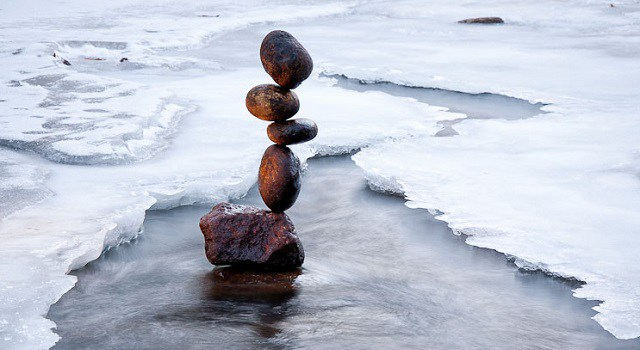
\includegraphics[width=0.7\linewidth]{Images/zen}
%\end{figure}
%\end{frame}

\begin{frame}{Zen State}
Zen = Stakeholders don't call you, unless it's your birthday


\begin{columns}[T] % contents are top vertically aligned
	\begin{column}[T]{5cm} % each column can also be its own environment
\begin{itemize}
	\item Productivity
	\item HR Availability
	\item Stability and predictability
	\item Scalability
	\item \textbf{Money}
\end{itemize}
	\end{column}
	\begin{column}[T]{5cm} % alternative top-align that's better for graphics
		\begin{figure}
			\centering
			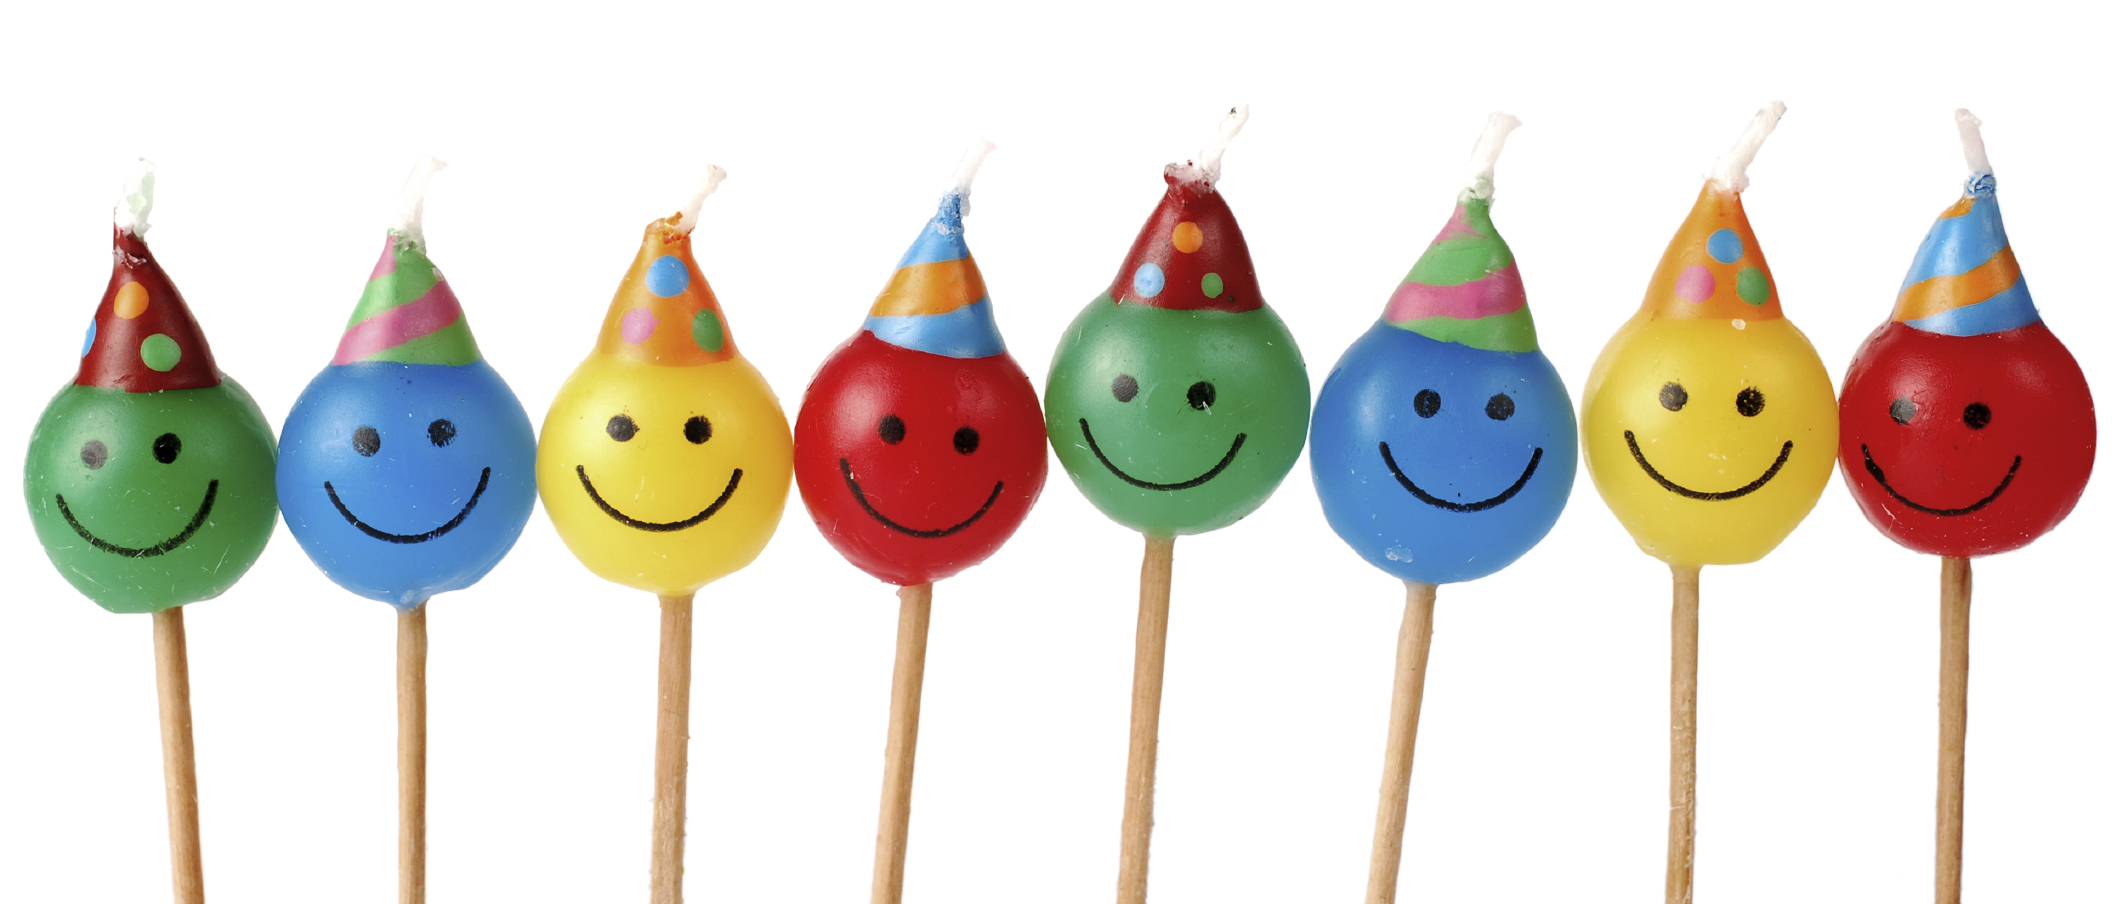
\includegraphics[width=\linewidth]{Images/candle-heads}
		\end{figure}
	\end{column}
\end{columns}
\end{frame}

\begin{frame}{Zen State}
Some sprints ago I had "birthdays" on daily basis

		\begin{figure}
			\centering
			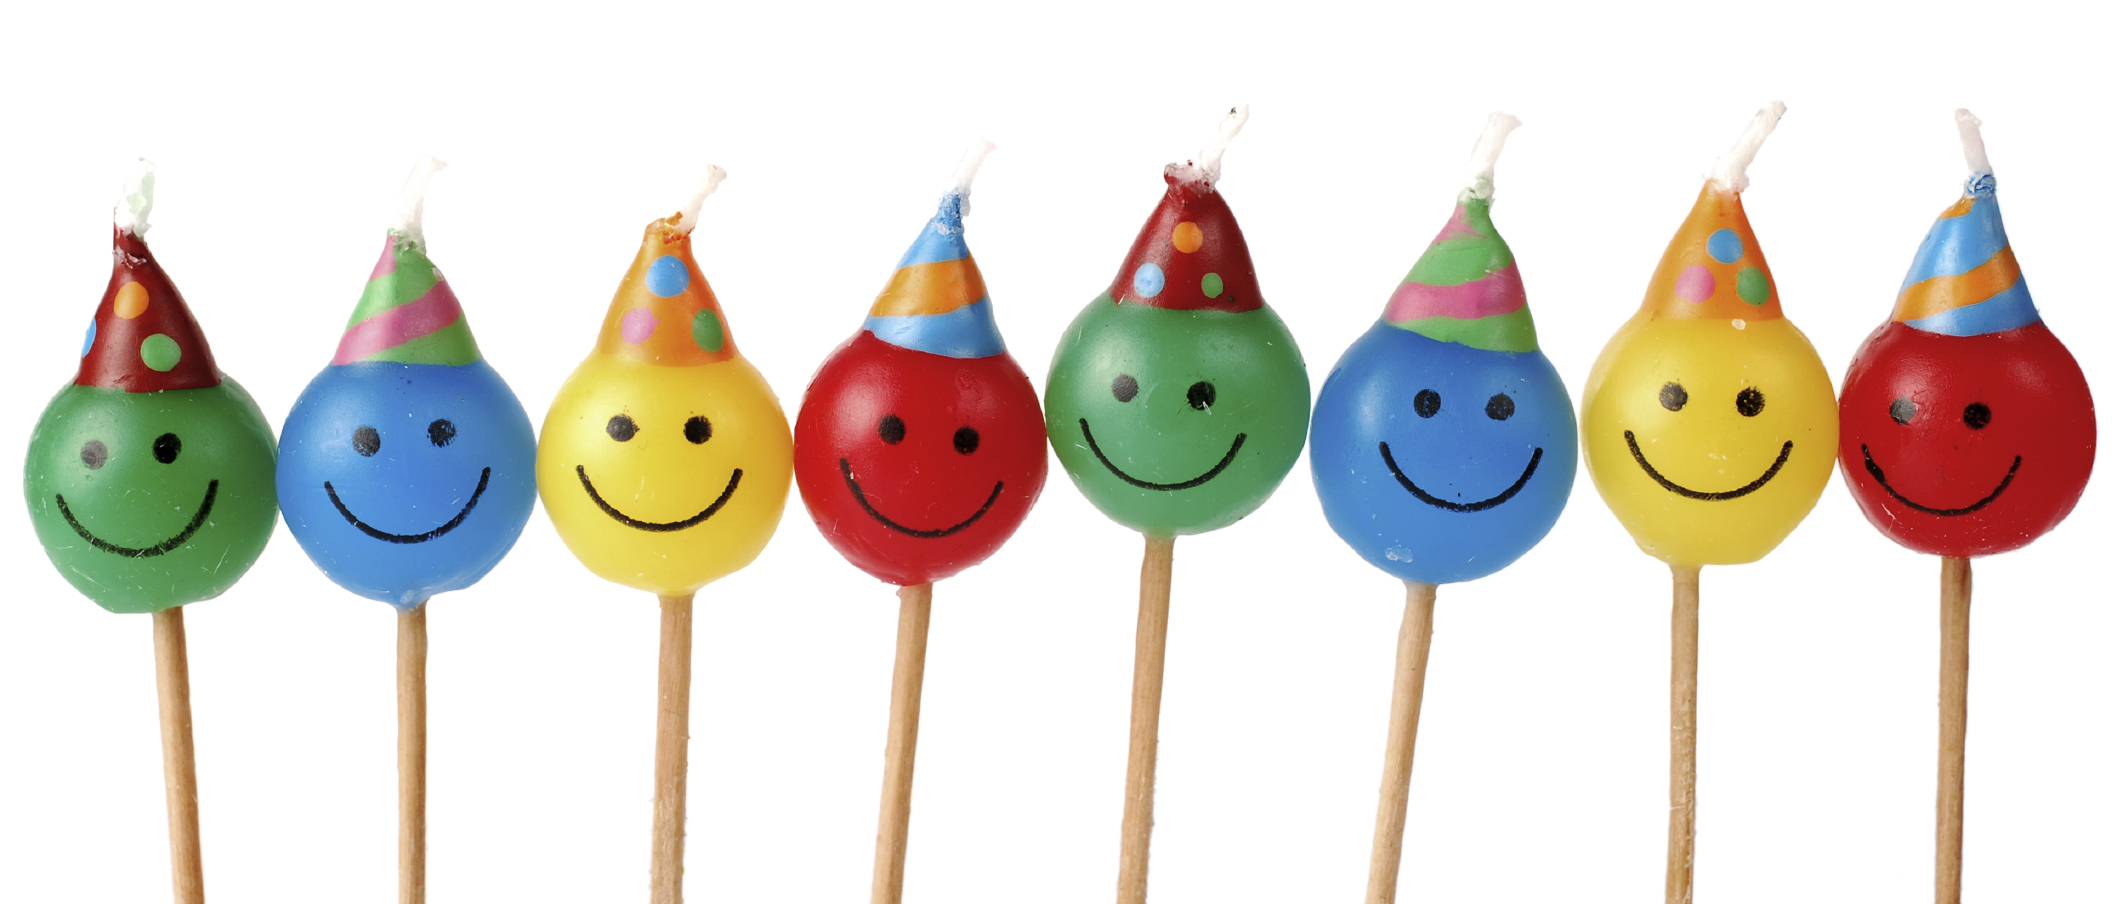
\includegraphics[width=\linewidth]{Images/candle-heads}
		\end{figure}

\end{frame}


\begin{frame}{How my birthdays started}
Please Víctor help us to do Microservices

\end{frame}


\begin{frame}{!Birthday}
Please Víctor help us to choose a \textbf{well known language}, with a \textbf{well known framework}, for achieving great \textbf{stability}, spending the \textbf{least money}, and take advantage of our \textbf{existing codebase}.

\begin{figure}
	\centering
	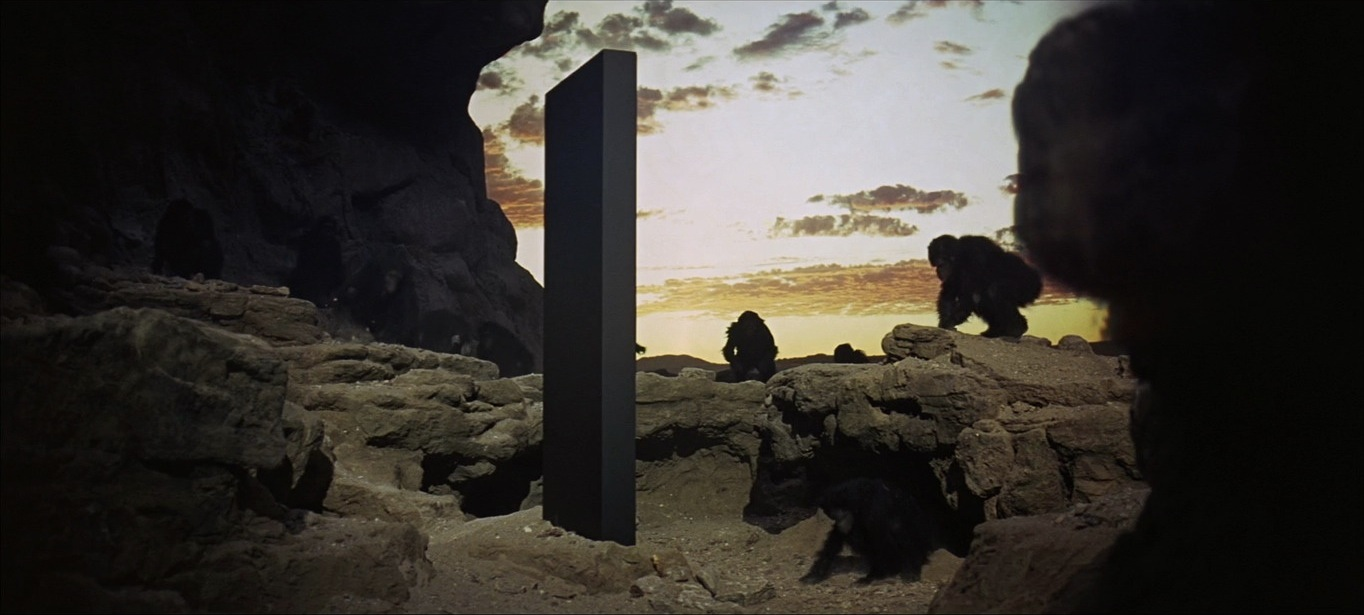
\includegraphics[width=\linewidth]{Images/monolith}
\end{figure}
\end{frame}

\section{Lesson 1: Microservices are a mindset revolution}
\begin{frame}{Monolith}
\begin{figure}
\centering
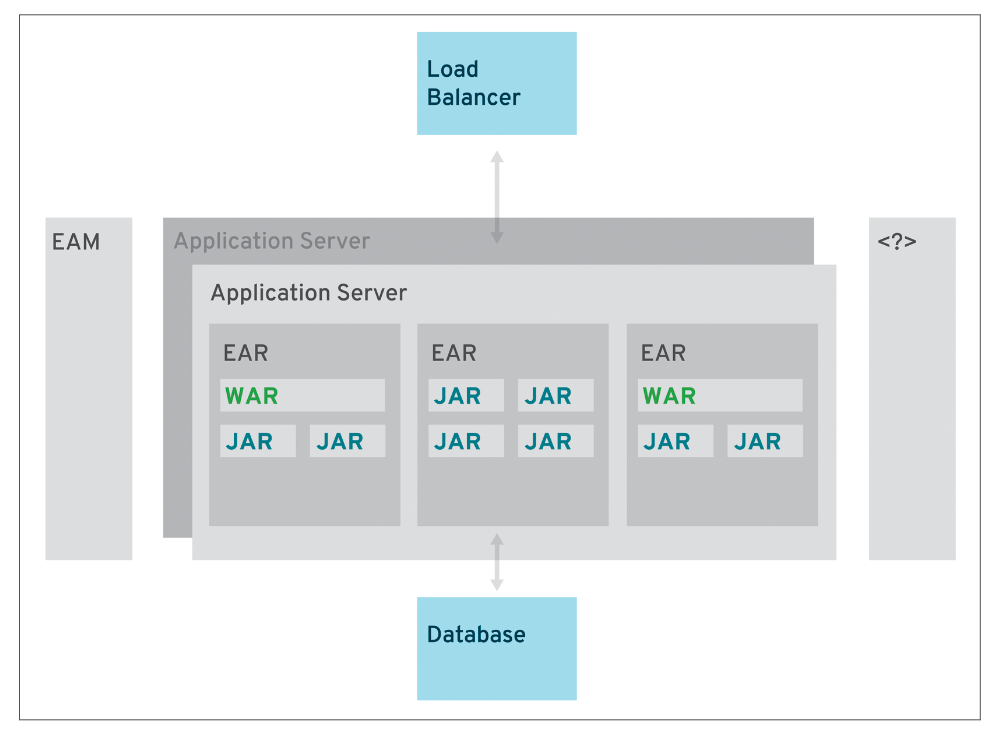
\includegraphics[width=0.7\linewidth]{Images/monolitos}
\caption{Regular monolith - Credits: Markus Eisele}
\end{figure}
\end{frame}

\begin{frame}{ESB}
\begin{figure}
\centering
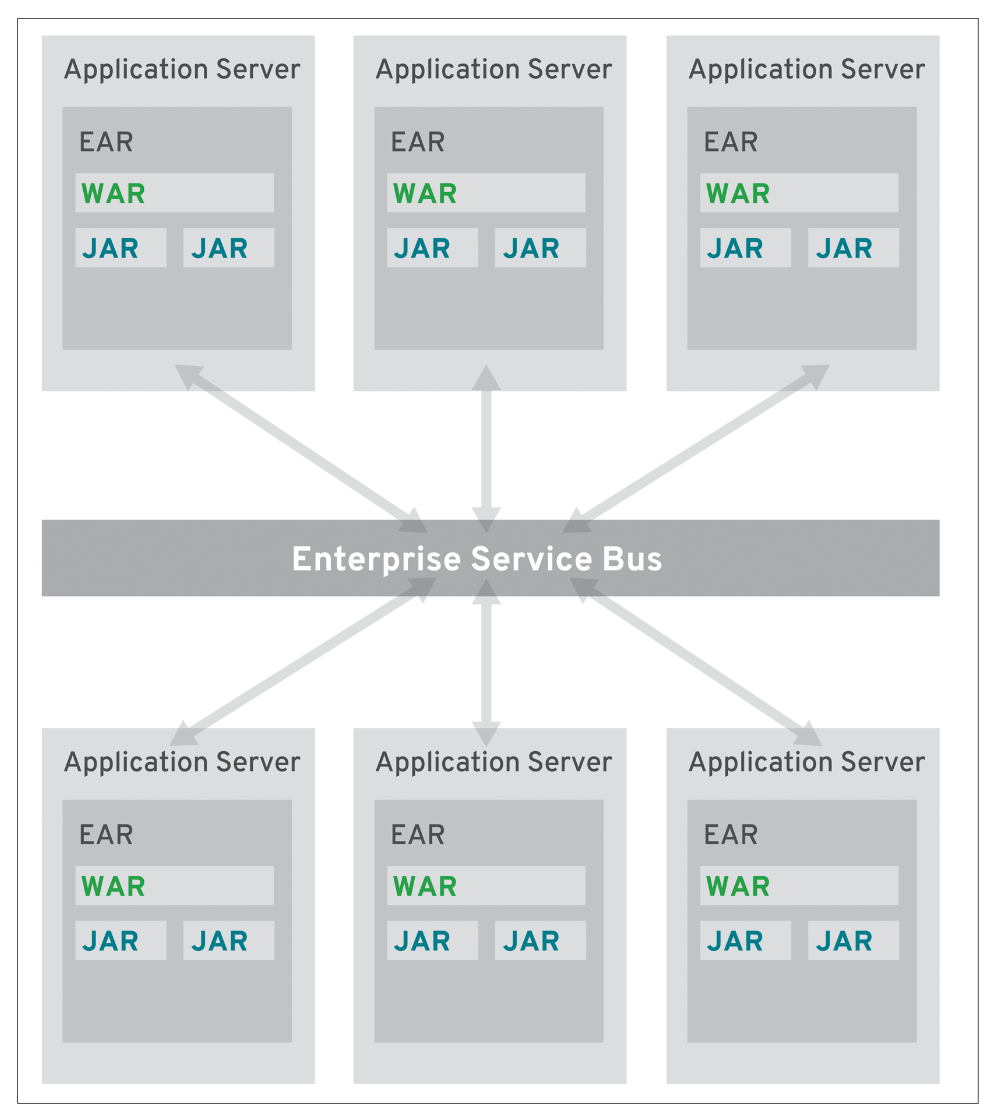
\includegraphics[width=0.5\linewidth]{Images/esb}
\caption{ESB - Credits: Markus Eisele}
\end{figure}
\end{frame}

\begin{frame}{Microservices}
\begin{figure}
\centering
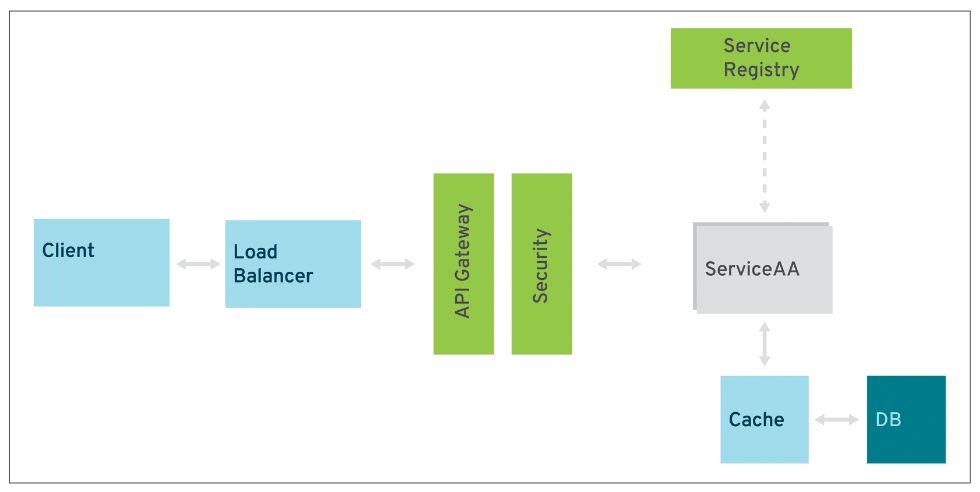
\includegraphics[width=\linewidth]{Images/microservicios}
\caption{Microservices - Credits: Markus Eisele}
\end{figure}
\end{frame}

\begin{frame}{Microservices}
Advantages
\begin{itemize}
	\item Small codebases
	\item Better software practices
	\item Fault tolerance
	\item Scalability
\end{itemize}
Disadvantages
\begin{itemize}
	\item Tooling overhead
	\item Debugging
	\item Distributed transactions
	\item Latency
	\item Dependency
\end{itemize}
\end{frame}


\begin{frame}{Microservices}
Disadvantages \\

\huge Hype Driven Development
\end{frame}


\section{Lesson 2: Functional Microservices are not the same for everybody}
\begin{frame}{How}
POC from Sr. to Jr.
\begin{itemize}
	\item Vert.x
	\item Spring Boot
	\item DropWizard
	\item Akka
	\item NodeJS
. . .
	\item JavaEE
\end{itemize}
\end{frame}

\begin{frame}{J2EE}
Jobs J2EE Guatemala 2018
\begin{figure}
	\centering
	
\includegraphics[width=\linewidth]{Images/javaee}
\end{figure}
\end{frame}

\begin{frame}{HR}
\begin{itemize}
	\item From the top five universities at country only three teach Java properly
	\item The other two teach .NET
	\item Sillicon Valley off-shores take best developers
\end{itemize}
\end{frame}


\section{Lesson 3: You don't need to be 100\% "microservice compliant"}
\begin{frame}{Microservices - JavaEE}
JavaEE is one of the most anti-hype frameworks\\

\huge J2EE 1.2 (December 12, 1999)
\end{frame}


\begin{frame}{Microservices - JavaEE}
Implementation
\begin{itemize}
	\item Iterative refactoring - Do it by waves
	\item Practical refactoring - Extract an already existing service 
	\item New services - New services talk to monolith
\end{itemize}
\end{frame}


\begin{frame}{Microservices - JavaEE}

\begin{figure}
	\centering
	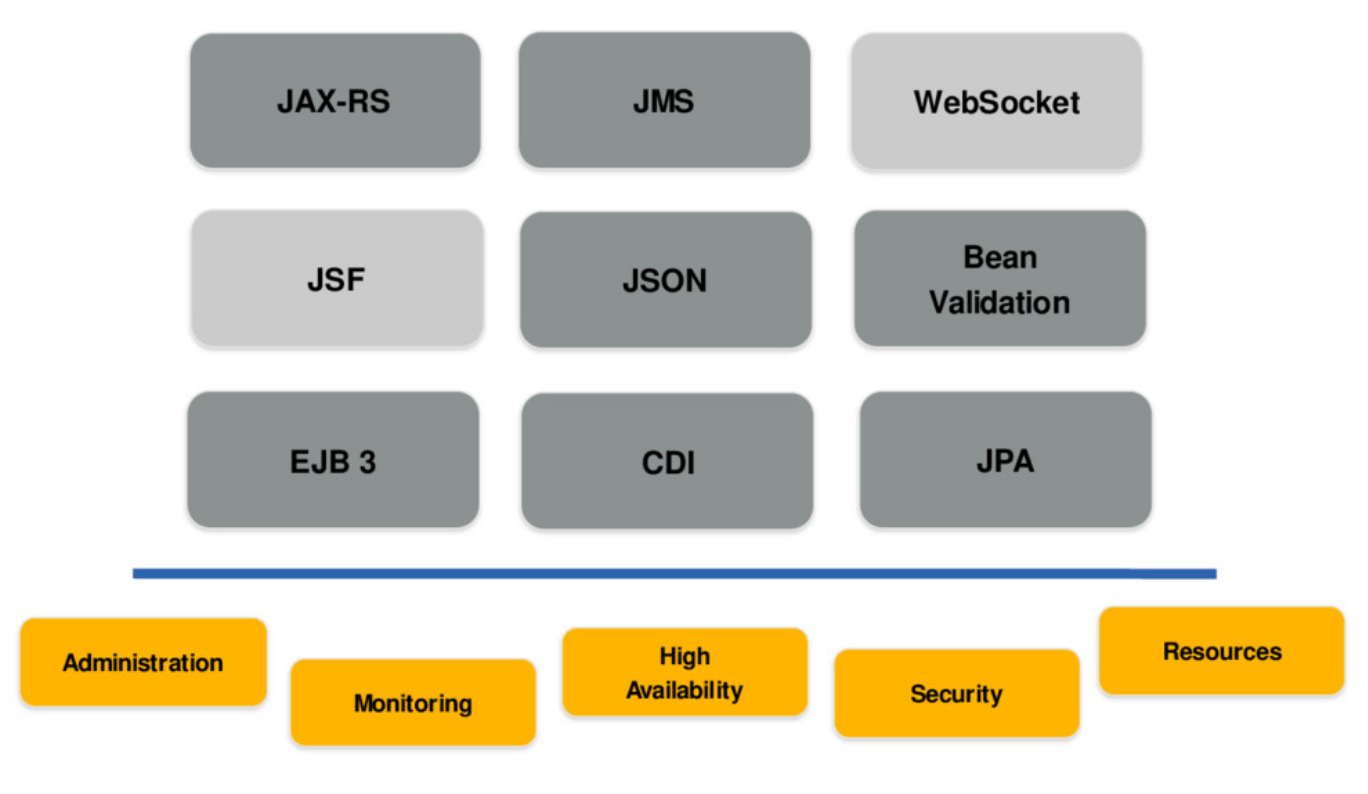
\includegraphics[width=0.9\linewidth]{Images/javaeemicropancake.png}
	\caption{JavaEE technologies - Credits: Reza Rahman}
\end{figure}
\end{frame}

\begin{frame}{Microservices - JavaEE}
\begin{figure}
	\centering
	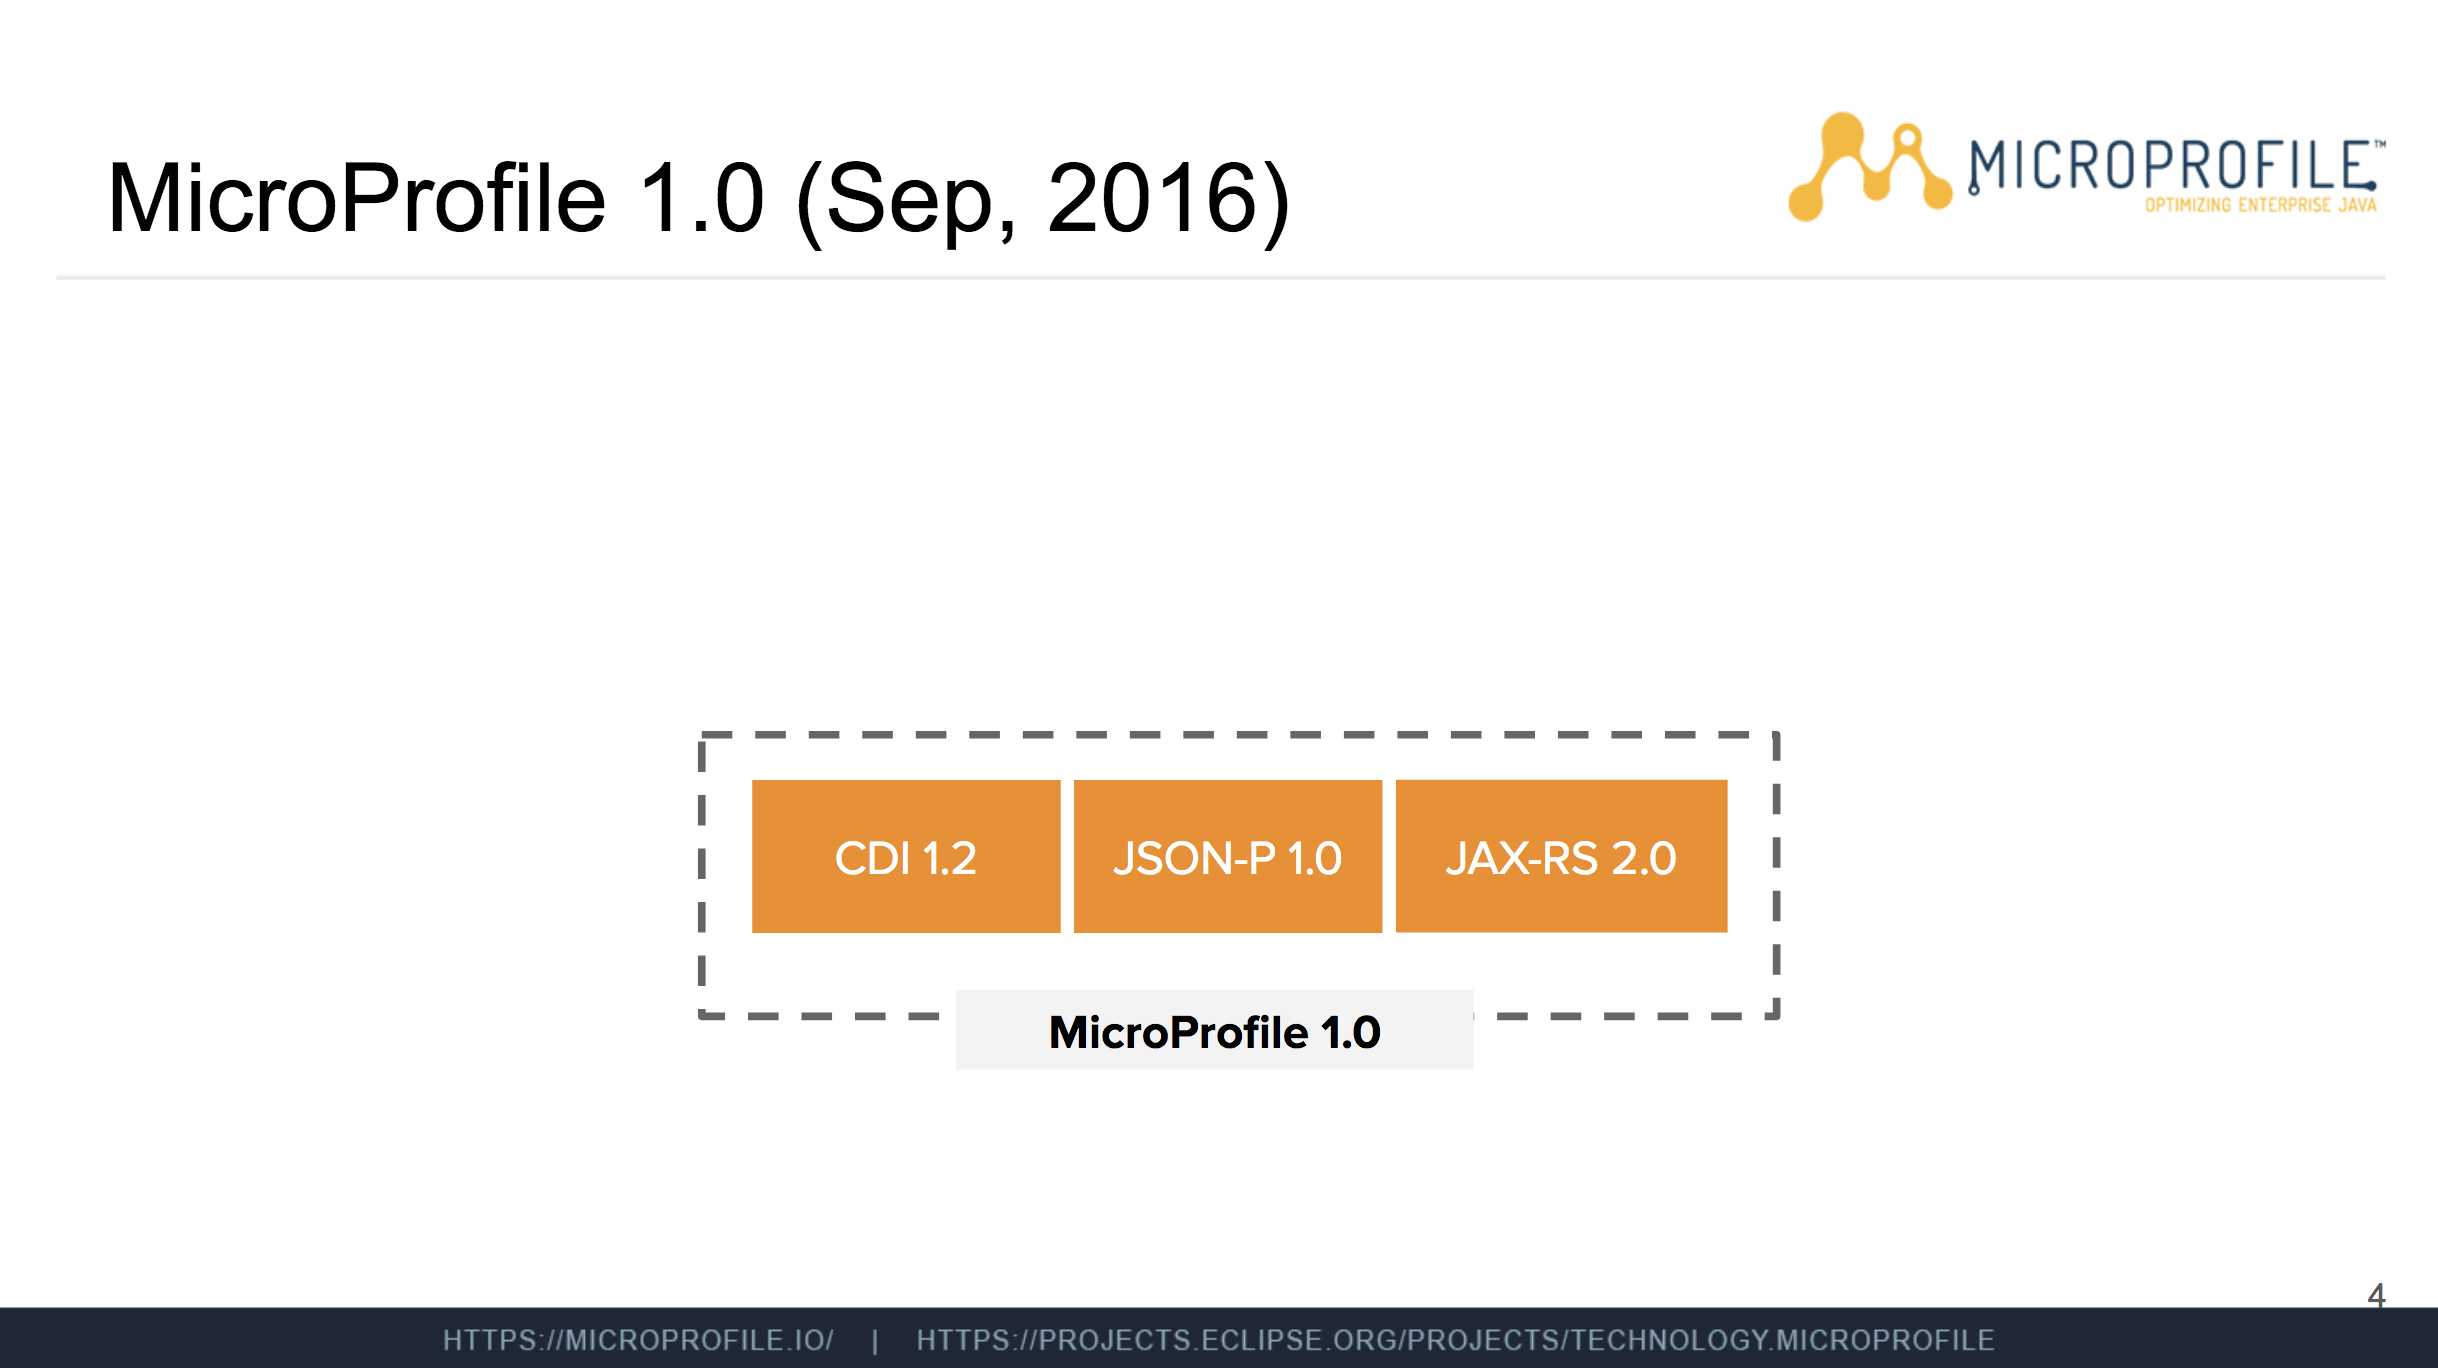
\includegraphics[width=\linewidth]{Images/mp1}
\end{figure}
\end{frame}

\begin{frame}{Microservices - JavaEE}
\begin{figure}
	\centering
	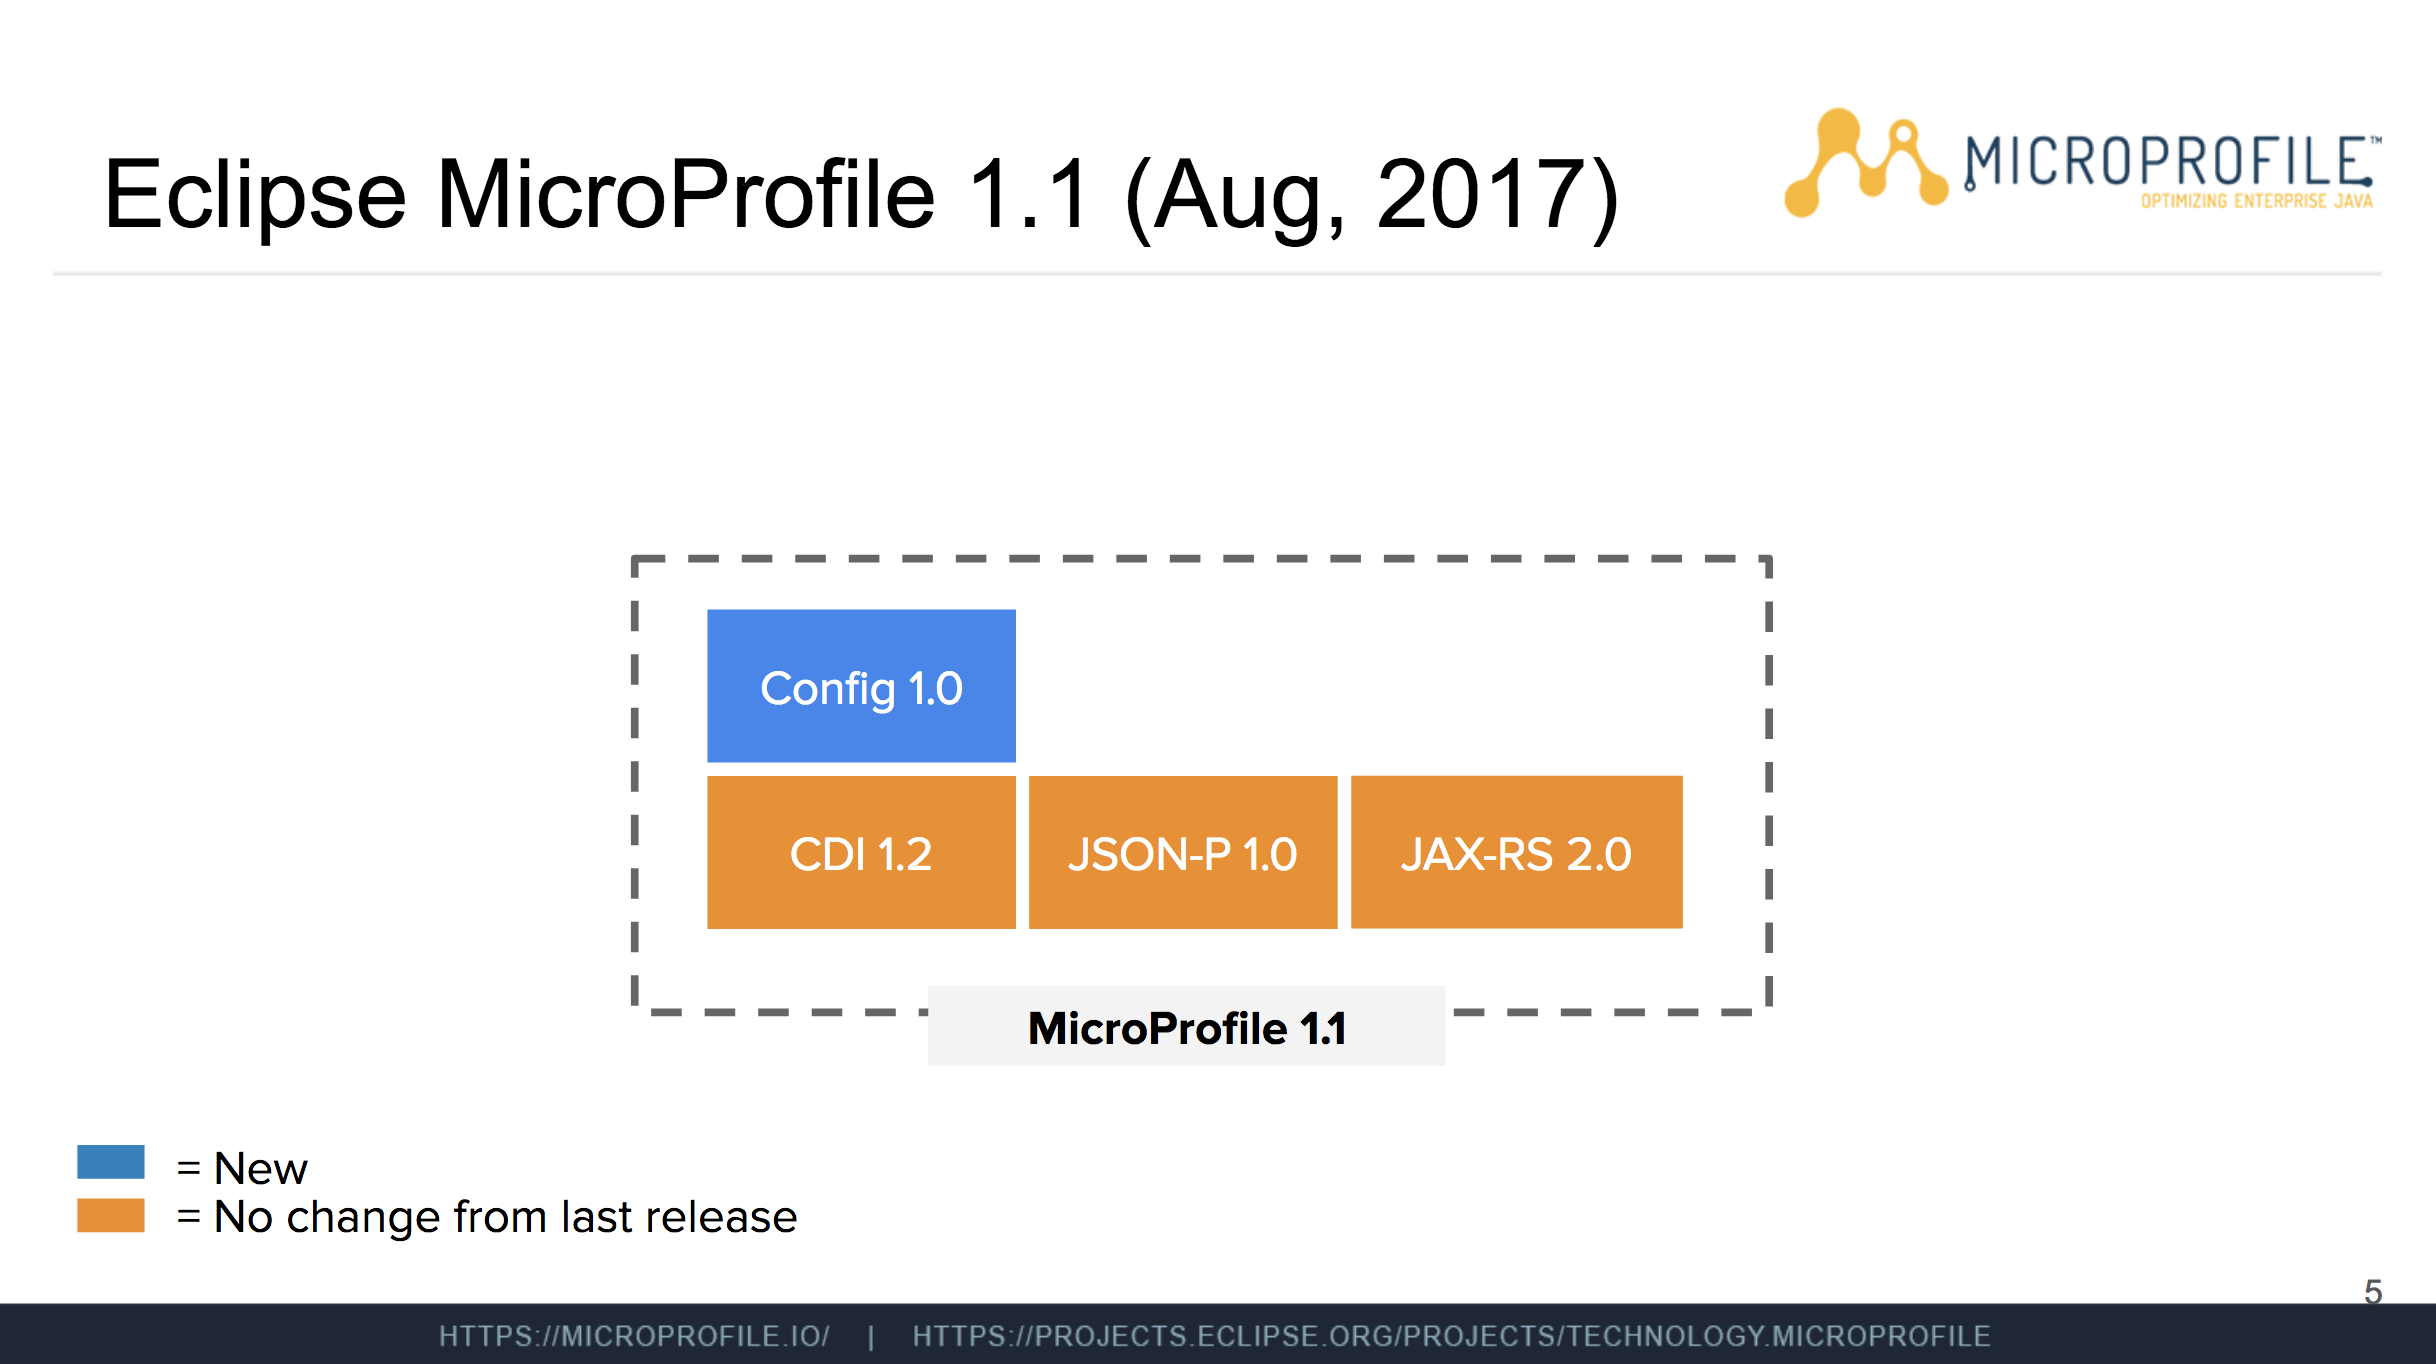
\includegraphics[width=\linewidth]{Images/mp2}
\end{figure}
\end{frame}

\begin{frame}{Microservices - JavaEE}
\begin{figure}
	\centering
	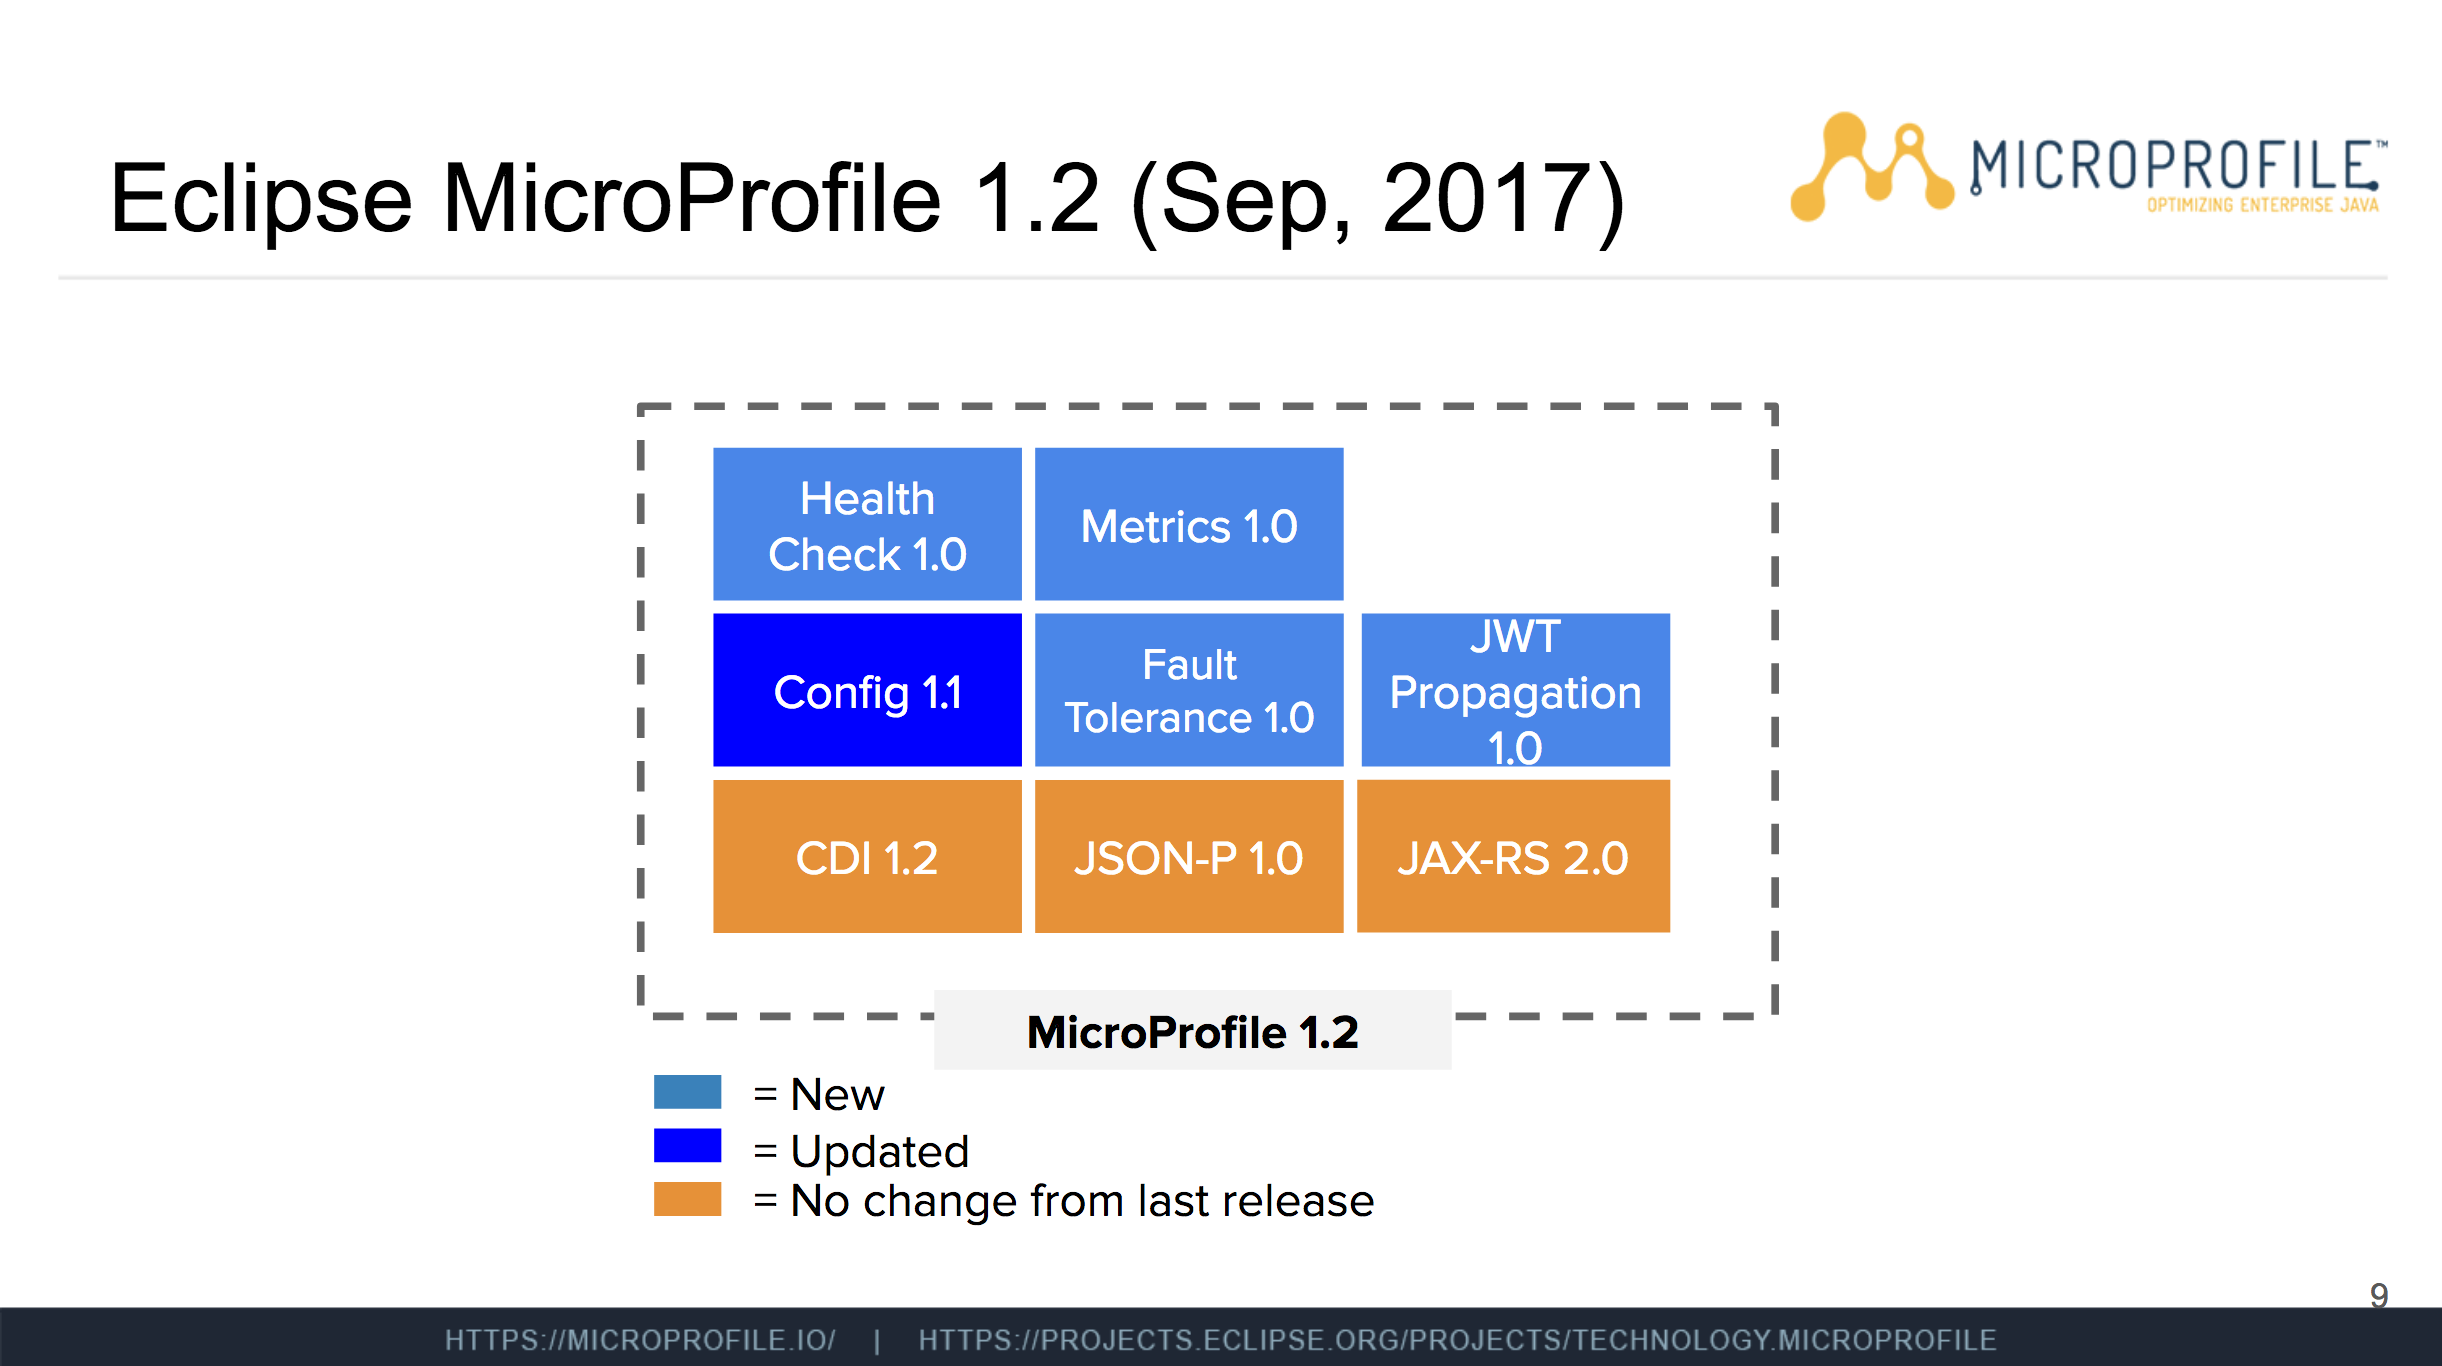
\includegraphics[width=\linewidth]{Images/mp3}
\end{figure}
\end{frame}

\begin{frame}{Microservices - Implementations}
\begin{itemize}
	\item Wildfly Swarm
	\item KumuluzEE
	\item Open Liberty
	\item TomEE
	\item \textbf{Payara Micro}
\end{itemize}
\end{frame}

\begin{frame}{Microservices - Payara}
Current target: Microprofile 1.2 

\begin{itemize}
	\item Microprofile 1.2 
	\item JavaEE Web Profile
	\item JCache
\end{itemize}

New deployments
\begin{itemize}
	\item Micro JavaEE server (CLI)
	\item Uber-Jar/Fat-Jar
\end{itemize}
\end{frame}



\section{Demo}
\begin{frame}{JavaEE Micro  - Demo}
\huge Java 8, JAX-RS, CDI, EJB, Microprofile

\normalsize  \url{https://github.com/tuxtor/payara-demo}\\
\normalsize  \url{https://github.com/tuxtor/omdb-demo}
\end{frame}

\begin{frame}{Payara Micro - Traditional JavaEE}
Granted
\begin{columns}[T] % contents are top vertically aligned
	\begin{column}[T]{3cm} % each column can also be its own environment
		\begin{itemize}
			\item EJB
			\item \textbf{JTA}
			\item JAX-RS
			\item CDI
		\end{itemize}
	\end{column}
	\begin{column}[T]{7cm} % alternative top-align that's better for graphics
\begin{figure}
	\centering
	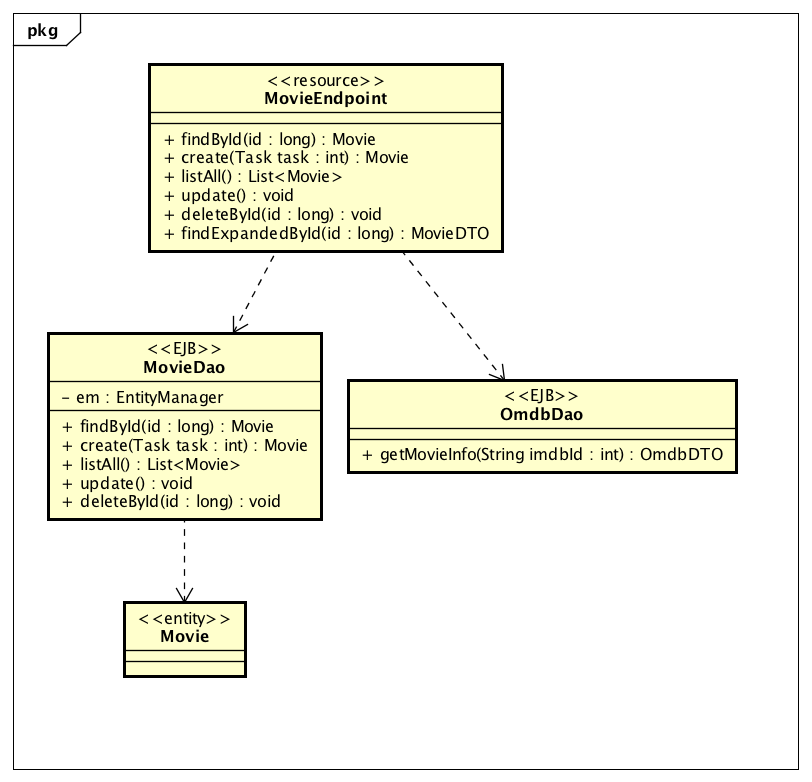
\includegraphics[width=\linewidth]{Images/democlass}
\end{figure}
	\end{column}
\end{columns}
\end{frame}

\begin{frame}{Payara Micro - Micro JavaEE}
\footnotesize MicroProfile: JAX-RS, CDI (Per service), Config, Fault Tolerance\\
Implementation: EJB, JTA (Per service)\\
Todo: Location, Deployment, Orchestation, Balancing, Consistency, Patterns
		\begin{figure}
			\centering
			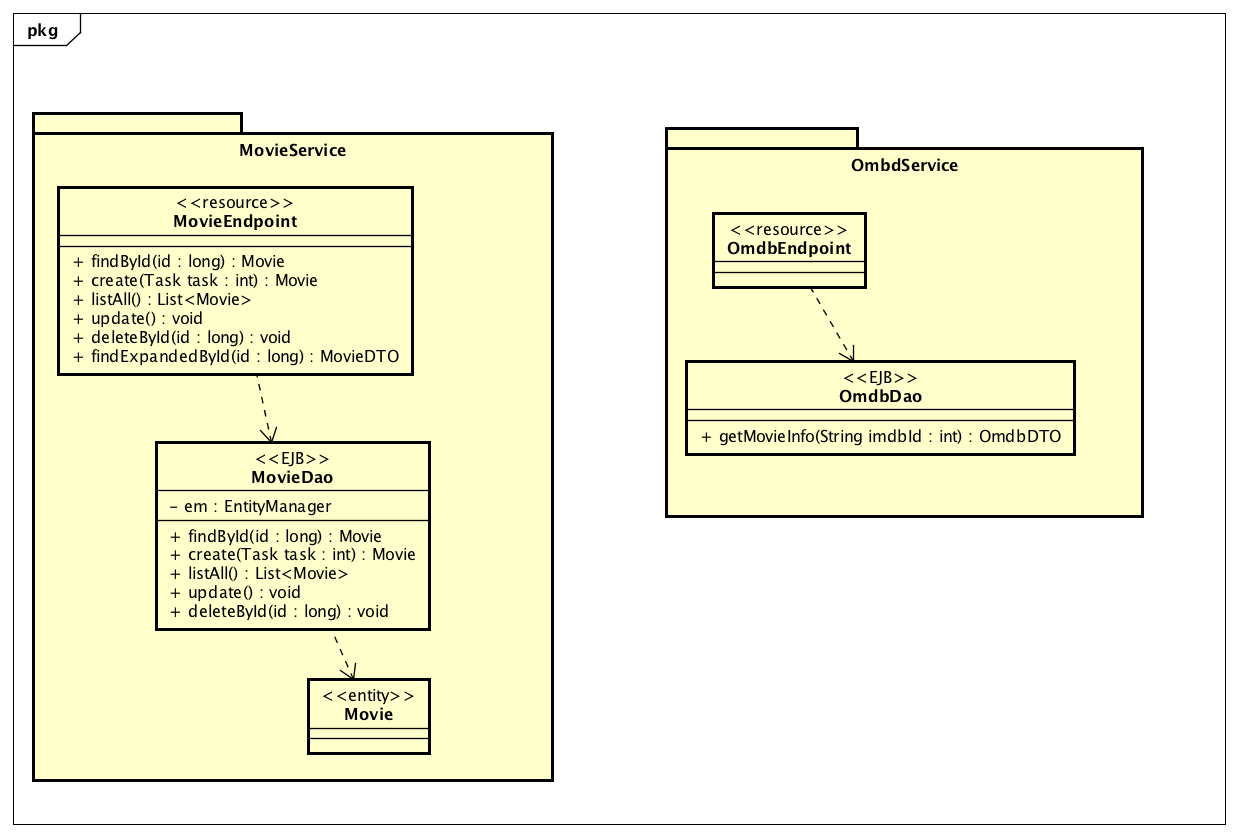
\includegraphics[width=0.95\linewidth]{Images/demomicro}
		\end{figure}

\end{frame}

\begin{frame}[fragile]{Config}
\begin{lstlisting}
@Inject
@ConfigProperty(name = "omdbservice.url")
String omdbDaemonServiceUrl;
\end{lstlisting}
\end{frame}

\begin{frame}{Fault tolerance}

\begin{itemize}
	\item Circuit Breaker
	\item Bulkhead
	\item Fallback
	\item Retry
	\item Timeout
\end{itemize}

\end{frame}


\begin{frame}[fragile]{Fault tolerance - Fallback, Timeout}
\begin{lstlisting}
@GET
@Path("/{id:[a-z]*[0-9][0-9]*}")
@Fallback(fallbackMethod = "findByIdFallBack")
@Timeout(TIMEOUT)
public Response findById(@PathParam("id") 
final String imdbId) {
...
}

public Response findByIdFallBack(@PathParam("id") 
final String imdbId) {
...
}
\end{lstlisting}
\end{frame}



\begin{frame}{Thank you}
\begin{itemize}
\item me@vorozco.com
\item http://vorozco.com
\item http://github.com/tuxtor/slides
\end{itemize}
\begin{center}

\includegraphics[width=0.1\linewidth]{Images/cclogo}
\\
This work is licensed under a Creative Commons Attribution-ShareAlike 3.0 Guatemala License.
\end{center}
\end{frame}
\end{document}

